\subsubsection{Detalhamento da Base Mecânica}~\label{sec::base_mec}%TODO
% Estevão: incluir desafios sob o ponto de vista mecânico
%TODO Estevão: descrever sistemas de fixação e ancoragem
%TODO Estevão: adicionar subseção de sistema de içamento e entrada dos
% equipamentos
%TODO Estevão: adicionar subseção do shutter
O estudo da base mecânica investigou primeiramente alguns conceitos baseados nos
graus de liberadade necessários para fornecer à base do robô todos os
posicionamentos necessários para revestimento de toda a pá, de acordo com os
estudos cinemáticos e dinâmicos. Os graus de liberdade são fornecidos através de
juntas prismáticas e rotacionais, que permitem o movimento do robô desde a
escotilha até o ponto de interesse para o início do processo de revestimento. A
seguir apresenta-se alguns conceitos analisados, em relação aos graus de
liberdade da base mecânica:

$\bullet$~\textbf{Base Prismática-Rotacional-Rotacional (P-R-R):}
  
  Neste conceito estudou-se a possibilidade de utilizar uma base com $3$ graus
  de liberdade: um prismático e dois rotacionais. O prismático seria composto
  por um trilho alinhado e paralelo ao eixo da turbina que transportaria o robô
  até a região próxima a pá. Uma junta rotacional e com eixo vertical orientaria
  a base nesta direção e uma junta perpedincular à primeira faria o
  posicionamento do elo de fixação da base do robô. A figura~\ref{fig::base_prr}
  ilustra este conceito.
    
  \begin{figure}[h!]
   \centering
   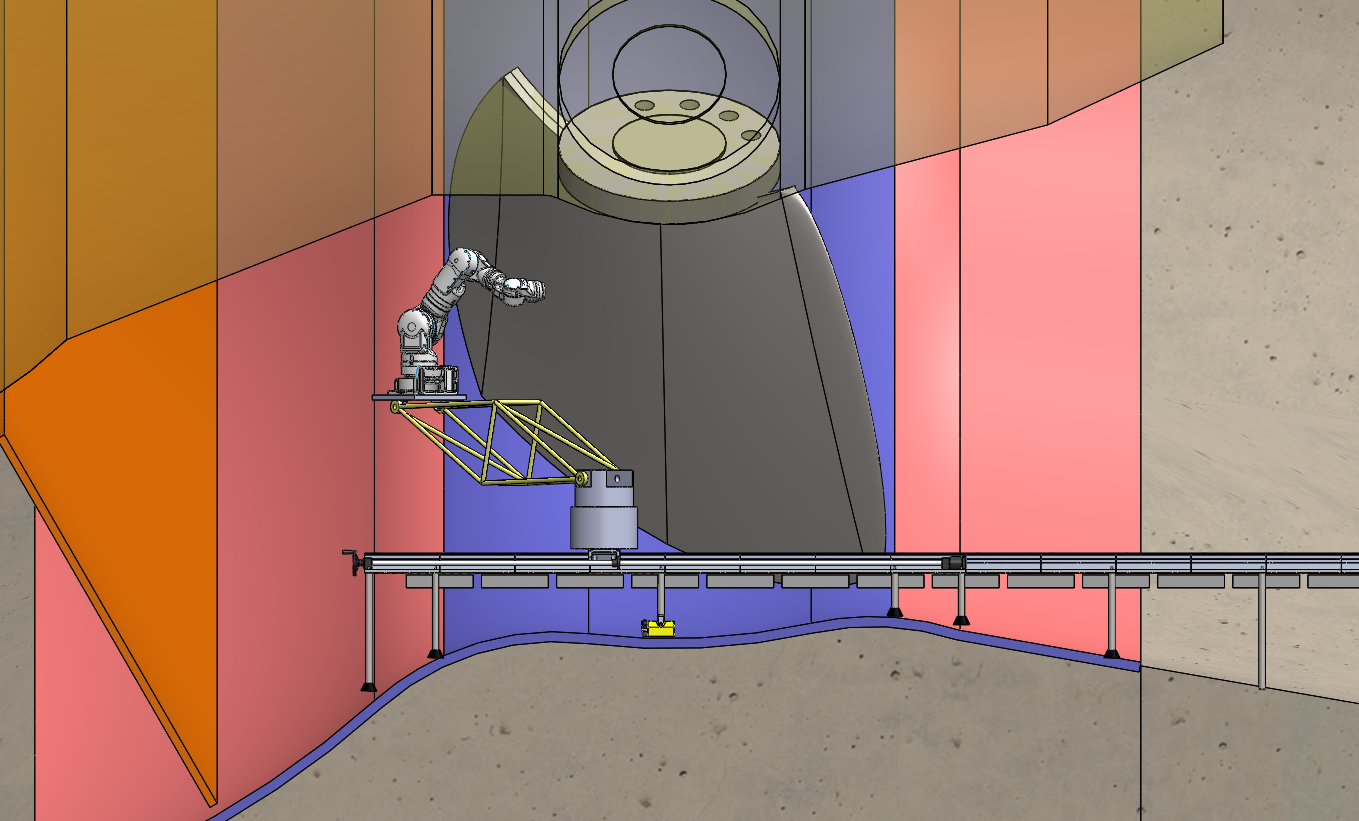
\includegraphics[width=0.8\columnwidth]{figs/bases/base_prr}
   \caption{Base Primático-Rotacional-Rotacional}
   \label{fig::base_prr}
\end{figure}

  Este conceito foi abandonado pela manobrabilidade reduzida da base, devido à
  configuração de juntas, o que levaria a posicionamentos difíceis ou até
  impossíveis de serem alcançados, dependendo do manipulador escolhido.
  
$\bullet$~\textbf{Base Prismática (P):}

  Este conceito consiste de um trilho (junta prismática) para o transporte do
  manipulador desde a escotilha até o ponto de interesse para revestimento na
  face anterior ou posterior da pá. Quando posicionado, remove-se a seção
  do trilho na direção que obstrui a rotação do rotor. Neste conceito,
  adiciona-se um grau de liberdade ao sistema utilizando a própria rotação do
  rotor, posicionando a pá em relação ao robô que é livre no trilho na direção
  do eixo da turbina e fixo nas outras direções. O procedimento para o
  revestimento seria o posicionamento do rotor, o posicionamento do robô no
  trilho, em relação a pá, a ancoragem do robô no ambiente e o revestimento da 
  região possível para aquela posição.
  Repete-se então este procedimento até ter toda a face processada e
  posiciona-se a próxima pá para revestimento, sem necessidade de mover ou
  desmontar a base do robô até todas as faces daquele lado estarem completas.  A
  figura~\ref{fig::base_p} ilustra este conceito.
  
  \begin{figure}[h!]
   \centering
   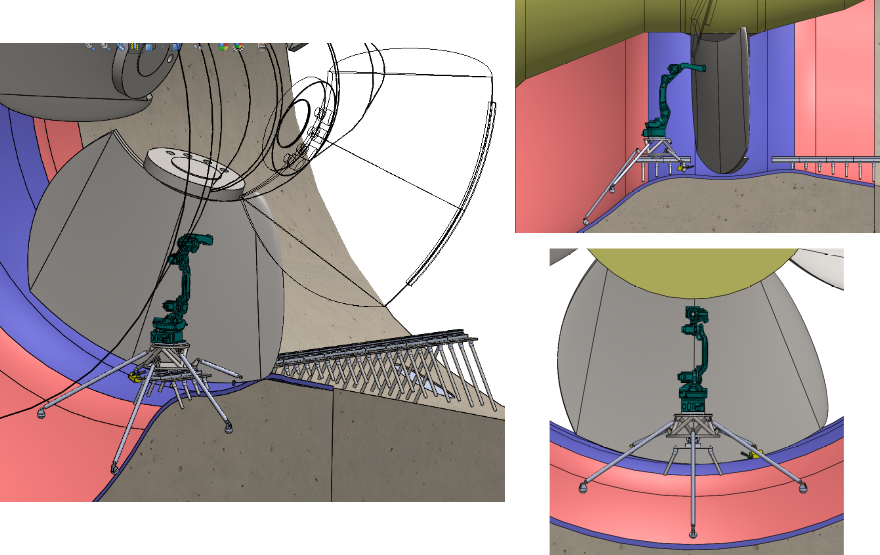
\includegraphics[width=0.8\columnwidth]{figs/bases/base_p}
   \caption{Base Primática}
   \label{fig::base_p}
\end{figure}

  A análise cinemática demonstrou que seriam necessárias muitas posições do
  rotor para completar uma face da pá. Há inclusive dificuldades operacionais e
  de segurança no procedimento de rotação do rotor que devem ser considerados. O
  rotor só pode ser girado manualmente, não fornecendo precisão no
  posicionamento da pá em relação a base. Por ser uma tarefa manual, deve-se ter
  procedimentos adequados de segurança para preservar tanto o operador quanto os
  equipamentos próximos. Estas preocupações tornam a solução pouco prática sob o
  ponto de vista operacional.

$\bullet$~\textbf{Base Prismática-Rotacional-Prismática (P-R-P):}

  Este conceito consiste de uma base composta por um trilho primário (junta
  prismática $1$), uma plataforma de base pivotada por mancal e rolamentos entre
  o trilho primário e secundário (junta rotacional) e um trilho secundário
  (junta prismática $2$). Montado o trilho primário alinhado ao eixo da turbina
  a base rotacional sobre o trilho primário, fixa-se o robo sobre a base
  rotacional. Esta base permitrá a montagem do trilho secundário apenas quando o
  robô atingir a região de interesse para revestimento. Quando posicionado o
  manipulador, monta-se então o trilho secundário alinhado ao plano paralelo a
  face da pá e ancora-se a base no ambiente. Desta forma, o robô pode-se
  movimentar ao longo de toda a extensão da pá por meio do trilho secundário e
  também se aproximar e se afastar da superfície da pá, por meio do trilho
  primário. 

\begin{figure}[h!]
   \centering
   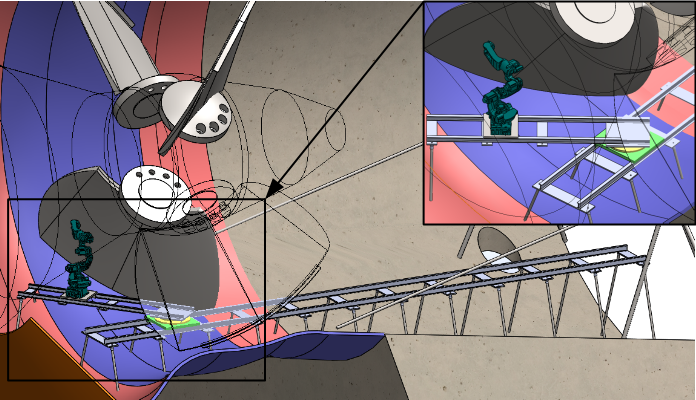
\includegraphics[width=0.8\columnwidth]{figs/bases/base_prp}
   \caption{Base Primática-Rotacional-Prismática}
   \label{fig::base_prp}
\end{figure}
  